\documentclass[cal1spr16Lectures.tex]{subfiles}

\begin{document}

\section[]{}

% % %
\subsection[5.2 Definite Integrals]{\S 5.2 Definite Integrals}
% % %

% % %
\begin{frame}{\S 5.2 Definite Integrals}\small
In \S 5.1, we saw how we can use Riemann sums to approximate the area under a curve.  However, the curves we worked with were all non-negative.
\begin{que} 
What happens when the curve is negative?
\end{que}
\end{frame}

% % % 
\begin{frame}
\begin{ex} 
Let $f(x)=8-2x^2$ over the interval $[0,4]$.  Use a left, right, and midpoint Riemann sum with $n=4$ to approximate the area under the curve.

\begin{center}
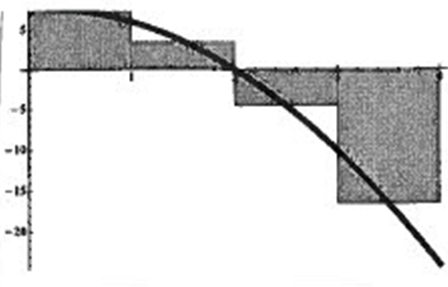
\includegraphics[scale=0.75]{pictures/5p2example}
\end{center} 
\end{ex}
\end{frame}

% % %
\subsubsection{Net Area}
% % %

% % %
\begin{frame}{\small Net Area}\footnotesize
In the previous example, the areas where $f$ was positive provided positive contributions to the area, while areas where $f$ was negative provided negative contributions.  The difference between positive and negative contributions is called the {\bf net area}.
\begin{dfn} 
Consider the region $R$ bounded by the graph of a continuous function $f$ and the $x$-axis between $x=a$ and $x=b$.  The {\bf net area} of $R$ is the sum of the areas of the parts of $R$ that lie above the $x$-axis minus the sum of the areas of the parts of $R$ that lie below the $x$-axis on $[a,b]$. 
\end{dfn}
\end{frame}

% % %
%\subsubsection{Definite Integral}
% % %

% % %
\begin{frame}%{\small Definite Integral}
\small
The Riemann sums give approximations for the area under the curve.  To make these approximations more and more accurate, we divide the region into more and more subintervals.  To make these approximations exact, we allow the number of subintervals $n \to \infty$, thereby allowing the length of the subintervals $\Delta x \to 0$.  In terms of limits:
\[
\text{Net Area}=\lim_{n \to \infty} \sum_{k=1}^n f(\overline{x}_k) \Delta x.
\]
\end{frame}

% % %
\subsubsection{General Riemann Sums}
% % %

% % %
\begin{frame}{\small General Riemann Sums}\footnotesize
Suppose $[x_0,x_1], [x_1,x_2], \dots, [x_{n-1},x_n]$ are subintervals of $[a,b]$ with $a=x_0 < x_1 < x_2 < \cdots < x_{n-1} < x_n=b$.  Let $\Delta x_k$ be the length of the subinterval $[x_{k-1},x_k]$ and let $\overline{x}_k$ be any point in $[x_{k-1},x_k]$ for $k=1,2,\dots,n$.  If $f$ is defined on $[a,b]$, then the sum
\[
\sum_{k=1}^n f(\overline{x}_k) \Delta x_{\alert k} = f(\overline{x}_1)\Delta x_{\alert 1} + f(\overline{x}_2)\Delta x_{\alert 2} + \dots + f(\overline{x}_n)\Delta x_{\alert n}
\]
is called a {\bf general Riemann sum for $\boldsymbol{f}$ on $\boldsymbol{[a,b]}$}.

\vspace{0.5pc}
{\bf Note:} In this definition, the lengths of the subintervals do not have to be equal.
\end{frame}

% % %
\subsubsection{The {\it Definite} Integral}
% % %

% % %
\begin{frame}{\small The {\it Definite} Integral}\footnotesize
As $n \to \infty$, all of the $\Delta x_k \to 0$, even the largest of these.  Let $\Delta$ be the largest of the $\Delta x_k$'s.  %Then we look for 
%\[
%\lim_{\Delta \to 0} \sum_{k=1}^n f(\overline{x}_k) \Delta x_k.
%\] 
%
%\vspace{-0.5pc}
\begin{dfn} The {\bf definite integral of $\boldsymbol{f}$ from $\boldsymbol{a}$ to $\boldsymbol{b}$} is
\[
\int_a^b f(x)\ dx = \lim_{\Delta  \to 0} \sum_{k=1}^n f(\overline{x}_k) \Delta x_k,
\]
where $f$ is a function defined on $[a,b]$.  When this limit exists -- over {\it all} partitions of $[a,b]$ and {\it all} choices of $\overline{x}_k$ on a partition -- $f$ is called {\bf integrable}. 
\end{dfn}
\end{frame}

% % %
\subsubsection{Evaluating Definite Integrals}
% % %

% % %
\begin{frame}{\small Evaluating Definite Integrals}\footnotesize
\begin{thm}
If $f$ is continuous on $[a,b]$ or bounded on $[a,b]$ with a finite number of discontinuities, then $f$ is integrable on $[a,b]$.
\end{thm}
See Figure 5.23, p.\ 325, for an example of a noncontinuous function that is integrable.

\vspace{0.5pc}
Knowing the limit of a Riemann sum, we can now translate that to a definite integral.
\begin{ex}
\[\displaystyle\lim_{\Delta  \to 0} \sum_{k=1}^n (4\overline{x}_k - 3)\Delta x_k\text{ on }[-1,4] \quad\equiv\quad \int_{-1}^4 (4x-3)\ dx\]
\end{ex}
\end{frame}

% % %
\begin{frame}\small
Without formally examining methods to evaluate definite integrals, we can use geometry.
\begin{exe} 
Using geometry, evaluate $\int_1^2 (4x-3)\ dx$. 

\vspace{0.5pc}
(\emph{Hint:}  The area of a trapezoid is $A=\frac{h(l_1+l_2)}{2}$, where $h$ is the height of the trapezoid and $l_1$ and $l_2$ are the lengths of the two parallel bases.)
\end{exe}
\end{frame}

% % %
\begin{frame}\footnotesize
\begin{exe} 
Using the picture below, evaluate the following definite integrals:
\[\text{1.\ } \int_0^a f(x)\ dx \qquad \text{2.\ } \int_0^b f(x)\ dx \qquad \text{3.\ } \int_0^c f(x)\ dx \qquad \text{4.\ } \int_a^c f(x)\ dx\]
\vspace{-2pc}

\begin{center}
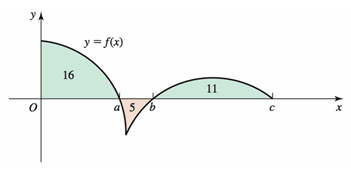
\includegraphics[scale=0.8]{pictures/Ch5Sect2_Exer31}
\end{center}
\end{exe}
\end{frame}

% % %
\subsubsection{Properties of Integrals}
% % %

% % %
\begin{frame}{\small Properties of Integrals}\footnotesize
\begin{itemize}
\item[1.] (Reversing Limits) $\int_b^a f(x)\ dx = -\int_a^b f(x)\ dx$

\vspace{0.75pc}
\item[2.] (Identical Limits) $\int_a^a f(x)\ dx = 0$

\vspace{0.75pc}
\item[3.] (Integral of a Sum) 

$\int_a^b (f(x)+g(x))\ dx = \int_a^b f(x)\ dx + \int_a^b g(x)\ dx$

\vspace{0.75pc}
\item[4.] (Constants in Integrals) $\int_a^b cf(x)\ dx = c \int_a^b f(x)\ dx$
\end{itemize}
\end{frame}

% % %
\begin{frame}{\small Properties of Integrals, cont.}\footnotesize
\begin{itemize}
\item[5.] (Integrals over Subintervals) If $c$ lies between $a$ and $b$, then
\[
\int_a^b f(x)\ dx = \int_a^c f(x)\ dx + \int_c^b f(x)\ dx.
\]

\item[6.] (Integrals of Absolute Values) The function $|f|$ is integrable on $[a,b]$ and $\int_a^b |f(x)|\ dx$ is the sum of the areas of regions bounded by the graph of $f$ and the $x$-axis on $[a,b]$.  (See Figure 5.31 on p.\ 329) 

\vspace{0.5pc}
\alert{(This is the total area, no negative signs.)}
\end{itemize}
\end{frame}

% % %
\begin{frame}\small
\begin{exe} 
If $\int_2^4 f(x)\ dx = 3$ and $\int_4^6 f(x)\ dx = -2$, then compute 
$\int_2^6 f(x)\ dx$. 
\end{exe}
\end{frame}

% % %
\subsubsection{Book Problems}
% % %

% % %
\begin{frame}
\begin{block}{5.2 Book Problems}
11-45 (odds), 67-74
\end{block}
\end{frame}

\end{document}